%!TEX root = draft.tex
\section{Empirical Analysis}
\label{sec:Analysis}

In this section, we describe key factors that impact edge formation in
real networks and analyze global structural properties of real networks,
a cumulative effect of edge formation mechanisms over time. Then, we briefly
contrast findings of empirical studies in sociology to common assumptions in
network modeling.

\subsection{Factors Influencing Edge Formation}
\label{subsec:factors}

We describe three factors --- preferential attachment, triadic closure \&
homophily --- that influence how individuals form links in real networks.
Compact statistical descriptors of global network properties
~\cite{newman2010networks} --- degree distribution, local clustering
coefficient \& attribute assortativity --- quantify the cumulative effect of these
factors on global network structure.

% pref attach
In the preferential attachment process \cite{simon1955class,
barabasi1999emergence}, nodes with higher degree receive links at a
faster rate because incoming nodes tend to link to well-connected nodes that
have more visibility. As a result, initial
differences in node connectivity get reinforced over time, giving rise to a
rich-get-richer effect. This phenomenon cumulatively leads to a heavy tailed
degree distribution, in which a small but significant fraction of nodes turn
into well-connected hubs.

% triadic closure
In the triadic closure phenomenon \cite{simmel1950sociology, newman2001clustering},
nodes with one or more common neighbors have an increased likelihood of forming a connection.
The local clustering coefficient of a node measures the prevalence of triadic closure in its
neighborhood; It is the probability that two randomly chosen neighbors of the node $i$
are connected: In directed networks, there are multiple definitions of a node's neighborhood:
The neighborhood of node $i$ can refer to the set of
nodes that link to $i$, set of nodes that $i$ links to or the union of both sets.
We define neighborhood to be the set of all nodes that link to
node $i$.

% \begin{equation}
%     C(i) = \frac{|\{(j,k) : j \in N(i), k \in N(i), (j,k) \in E\}|}{|N(i)|(|N(i)|-1)}
% \end{equation}

% Homophily and Assortativity
Real attributed networks tend to exhibit homophily
\cite{mcpherson2001birds}, the phenomenon in which similar nodes are more likely
to be connected than dissimilar nodes. The assortativity coefficient ~\cite{newman2002assortative}
$r \in [-1, 1]$, measures the level of homophily (or heterophily) in an attributed network with
categorical nodal attribute $B = \{b_1...b_l\}$.
It is defined as the ratio between the observed modularity and the maximum possible
modularity with respect to attribute $B$
Intuitively, it compares the observed fraction of edges between nodes with the same attribute
value to the expected fraction of edges between nodes with same
attribute value if the edges were rewired randomly.
High assortativity implies that nodes with the same
attribute value are more likely to be connected than nodes with different attribute values.

% \begin{equation}
%     r = \frac{Q_B}{Q^{\mbox{max}}_B} = \frac{\sum\limits_{b \in B} e_{bb} - \sum\limits_{b \in B} e_{b.}e_{.b}}{1 - \sum\limits_{b \in B} e_{b.}e_{.b}} \label{atty}
% \end{equation}

% conclude
Preferential attachment, triadic closure and homophily not only effect how individuals
form connections at the local level but also have a cumulative effect on the
global structural properties of real networks.

\subsection{Observations from Network Data}
In this subsection, we analyze global structural properties of the bibliographic network datasets
listed in \Cref{sec:Datasets}. We identify regularities in key global network properties:
indegree distribution, network growth rate, clustering and attribute mixing patterns.

Citation networks exhibit highly skewed, heavy tailed indegree distributions.
This implies that most papers receive zero or a few citations, but a small but
significant percent of the nodes turn into popular hubs that receive many
citations.
Lognormal fits describe the indegree distribution of all network datasets,
well consistent with Broido \& Clauset's \cite{broido2018scale} observation
that most real-world scale free networks are rare; The parameters of the lognormal
fits are listed in \cref{table:netstats}.
% In our proposed model, we
% incorporate preferential attachment using a random walk based edge formation
% mechanism to generate networks with heavy tailed indegree distribution.

The average outdegree of nodes that join real-world networks tends to increase
as functions of network size and time. This phenomenon densifies networks and shrinks their
diameter over time; Leskovec et al. \cite{leskovec2005graphs} show that
densification in many real networks exhibit a power law relationship between the
number of edges $e(t)$ and nodes $n(t)$ at time $t$: $e(t) \propto
n(t)^{\alpha}$. \Cref{table:netstats} lists the densification power law exponent $\alpha$ in
the network datasets. In our proposed model, we increase the outdegree of incoming nodes
at a linear or superlinear rate to account for the accelerated network growth
observed in real networks.
% as shown in ~\Cref{fig:empirical_analysis}.
\begin{table}[!h]
 \center
 {
  \begin{tabular}[c]{lrrrr} \toprule
  Network Dataset &  \texttt{LN} $(\mu, \sigma)$ & \texttt{DPL} $\alpha$       &  Avg. ${\texttt{LCC}}$  & \texttt{AA} $r$   \\ \midrule
  \texttt{USSC}     &   (1.19, 1.18) & 2.32     & 0.12    & -     \\
  \texttt{HEP-PH}   &   (1.32, 1.41) & 1.67     & 0.12    & -     \\
  \texttt{Semantic} &   (1.78, 0.96)  & 1.58     & 0.06    & -     \\   \midrule
  \texttt{ACL}      &   (1.93, 1.38)  & 1.43     & 0.07    & 0.07     \\
  \texttt{APS}      &   (1.62, 1.20)  & 1.26     & 0.11    & 0.44     \\
  \texttt{Patents}  &   (1.10, 1.01)   & 1.94     & 0.04    & 0.72    \\
  % \texttt{PYPI}         & 1.208     & 0.0524    & 0.692   & a\\
   \bottomrule
  \end{tabular}
  \vspace{1mm}
  \caption{Network properties: lognormal (\texttt{LN}) degree distribution mean \& standard deviation $(\mu, \sigma)$,
  densification power law (\texttt{DPL}) exponent $\alpha$, average local clustering coefficient (${\texttt{LCC}}$)
  and attribute assortativity (\texttt{AA}) coefficient of six network datasets.}
  \label{table:netstats}
 }
\end{table}

Real-world networks tend to exhibit high average local clustering, as shown in
\Cref{table:netstats}. Local clustering quantifies the extent to which triadic
closure influences underlying edge formation mechanisms.
% Coupled with small average path length, it also leads
% to the small-world phenomenon, in which two randomly picked nodes in large,
% sparse networks are connected by a short path with high probability.
As shown
in~\Cref{fig:cc_dc}, the distribution over local clustering in
these networks is skewed. While models  \cite{klemm2002highly,holme2002growing}
that rely on triangle closing mechanisms preserve \textit{average} local clustering,
our experiments indicate that richer edge formation mechanisms are necessary to
preserve the skewed clustering distributions of real networks accurately.
\begin{figure}[!h]
 \centering
 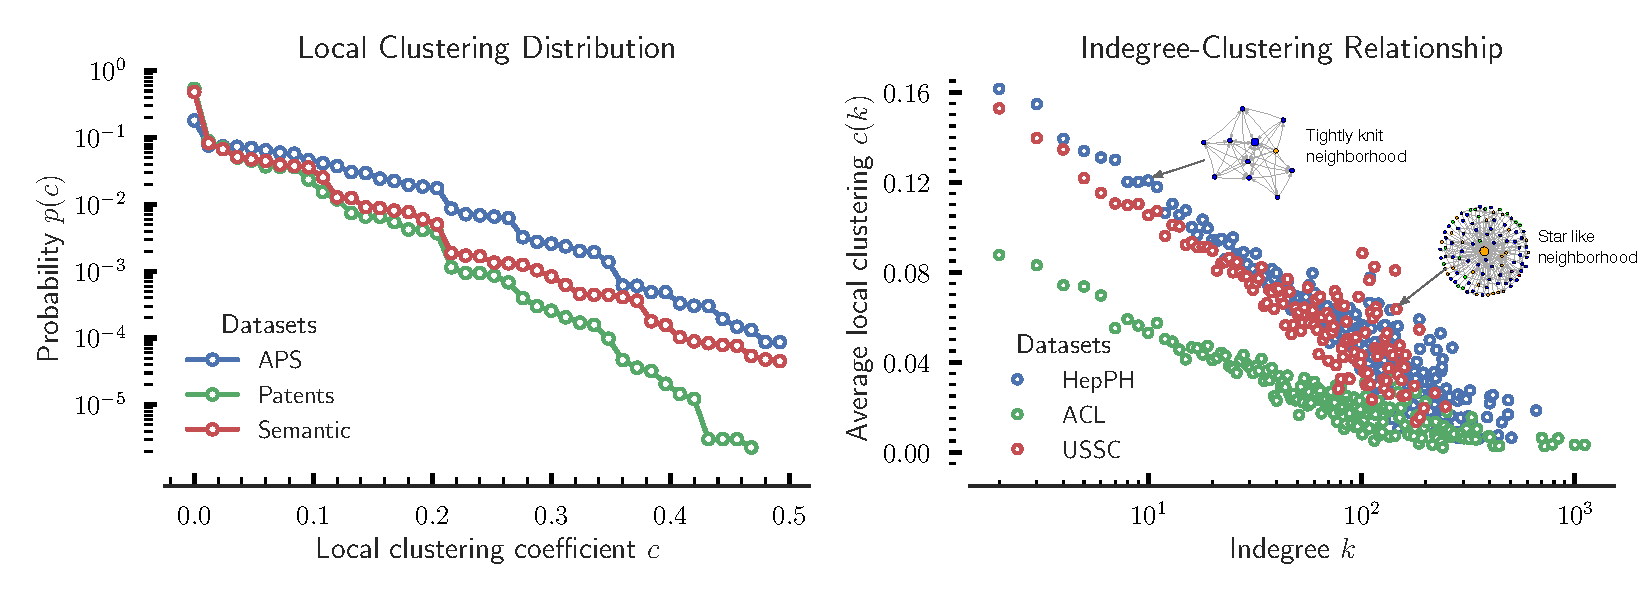
\includegraphics[width=\columnwidth]{cc_analysis}
 \caption{
    Local clustering in real networks have common characteristics:
    skewed local clustering distribution (left subplot) and a negatively correlated
    relationship between indegree and average local clustering (right subplot).
 }
 \label{fig:cc_dc}
\end{figure}

The bivariate relationships between indegree and clustering in \cref{fig:cc_dc}
show that average local clustering decreases as a function of indegree. Low
indegree nodes have small, tightly knit neighborhoods and high indegree
nodes tend have large, star-shaped neighborhoods.
% In~\Cref{sec:Proposed Model}, we propose a edge formation mechanisms that explains
% the emergence of degree-clustering relationships observed in real networks.
\begin{figure}[!h]
 \centering
 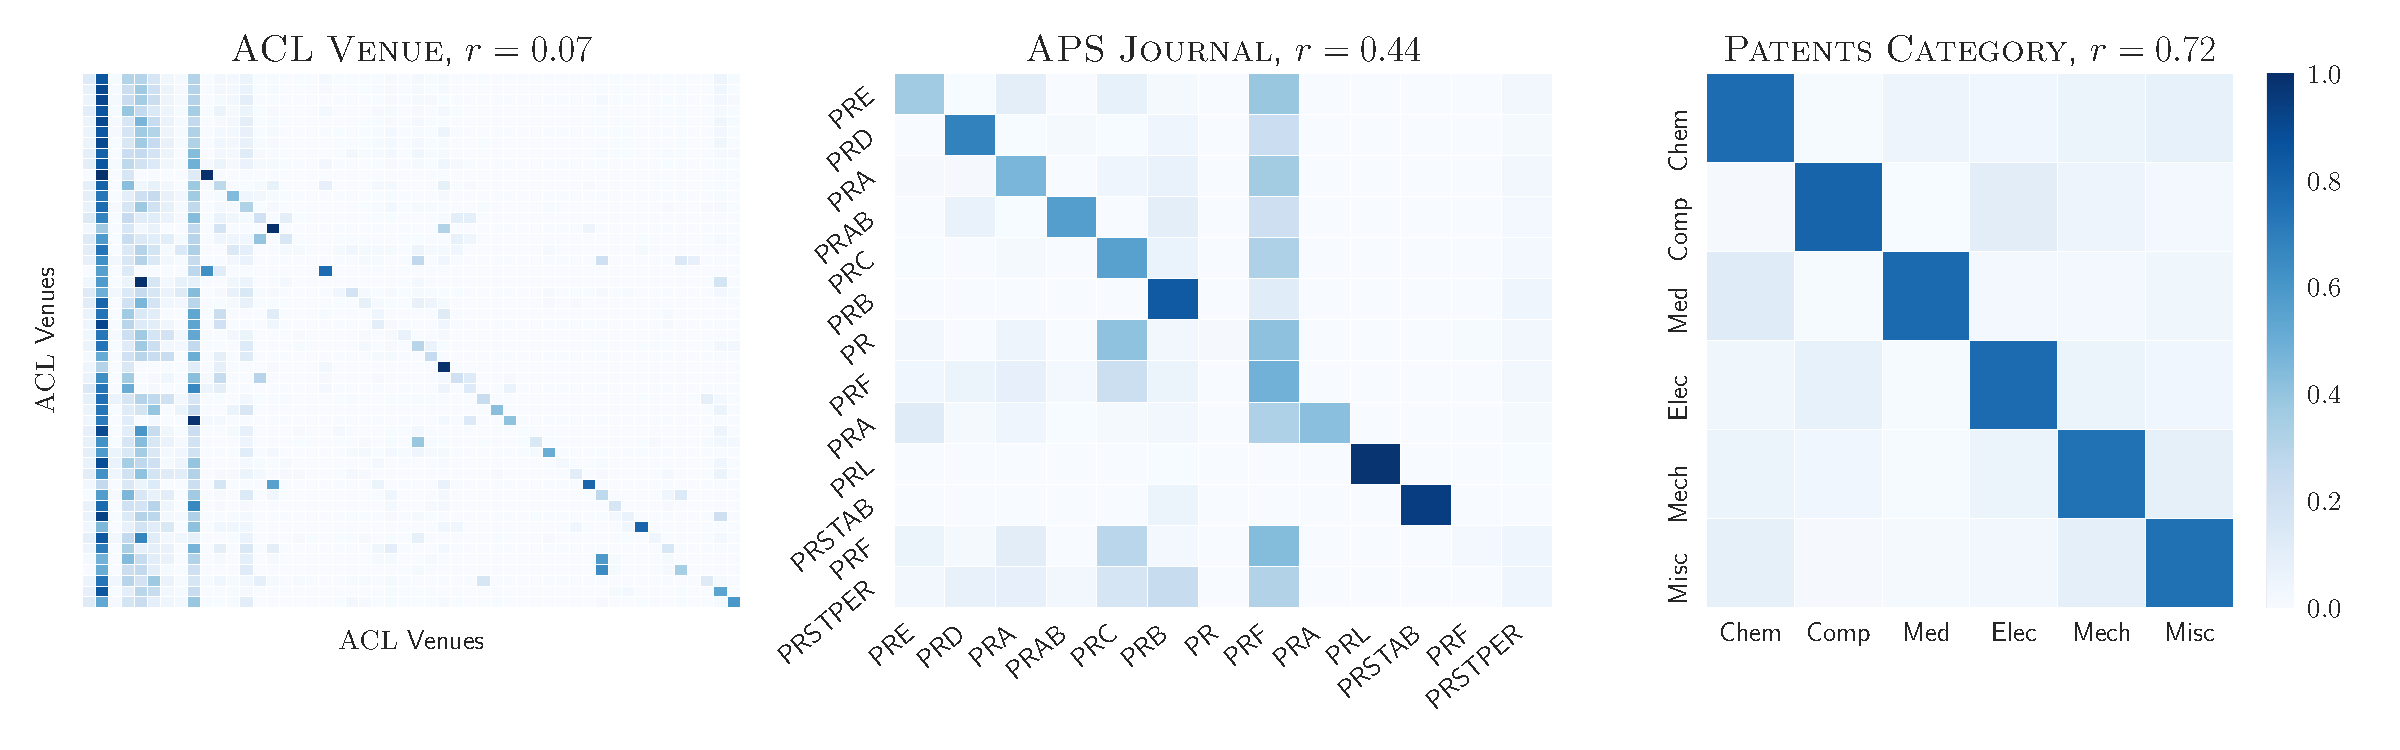
\includegraphics[width=\columnwidth]{mixing_v3}
 \caption{
    Attributed networks exhibit varying levels of homophily. The subplots
    illustrate the mixing patterns in \texttt{APS} and \texttt{Patents} w.r.t.
    attributes \texttt{Journal} ($r=0.44$) and \texttt{Category} ($r=0.72$) respectively.
 }
 \label{fig:mixing}
\end{figure}

Attributed networks such as \texttt{ACL}, \texttt{APS} \& \texttt{Patents} exhibit
varying level of homophily, as shown in \Cref{fig:mixing}, with assortativity
ranging from $0.07$ to $0.72$. The magnitude of the attribute assortativity
signifies the extent to which attribute similarity influences edge formation. Indeed,
homophilic preferences at the local level can lead to networks that have relatively
dense clusters of similar nodes. We model edge formation as a function of attribute
similarity to generate networks with varying attribute mixing patterns.

\subsection{Insights from Sociological Studies}

Sociological studies on network formation provide information about factors that
influence how individuals form edges in real-world networks.
Empirical studies
\cite{35626,block2014multidimensional} that investigate
the interplay between triadic closure and homophily in evolving networks
indicate that \textit{both} structural proximity and homophily are statistically
significant factors that influence edge formation. While homophilic preferences
\cite{mcpherson2001birds} induce edges between similar nodes,
structural factors (e.g. network distance) act as constraints that restrict
edge formation to structurally proximate nodes (e.g. friend of a friend).
Furthermore, extensive work \cite{simon1972theories,gigerenzer1996reasoning,lipman1995information}
on individual decision making establish that individuals are \textit{boundedly}
rational actors. That is, individuals make decisions under constraints of limited
information, cognitive capacity and time. Boundedly rational actors employ simple rules
to form edges under constraints of limited nodal information and partial network access.
For example, a researcher cites academic papers without knowledge of or access
to the entire literature in her or his field.

Based on these observations, an faithful characterization of edge formation in real-world
networks necessitates bias towards nodes that are similar, proximate or
well-connected under constraints of limited information and network access.
Existing preferential attachment or fitness-based models
\cite{dorogovtsev2000structure,kim2017effect,singh2017relay,barabasi1999emergence}
make two assumptions that are inconsistent with studies on edge formation formation
in evolving networks.
First, by assuming that successive edge formations are independent, these model
disregard the effect of triadic closure and structural proximity. Second, they
implicitly require incoming nodes to have complete network access (e.g., connect
to any node) or explicit knowledge of one or more properties (e.g., fitness) of

To summarize, citation networks tend to be homophilic networks that
undergo accelerated network growth and exhibit regularities in structural
properties: tailed indegree distributions, skewed local clustering distributions,
negatively correlated degree-clustering relationship and varying mixing patterns. These global properties
are a cumulative effect of individuals' edge formation decisions under resource
constraints.

% The regularities in
% the  global structure of citation networks perhaps suggest that individuals use
% similar edge formation mechanisms.

Next, we propose a growth model that unifies multiple
sociological phenomena to explain how \textit{local} factors that affect
edge formation lead to the emergence of global structural properties
observed in real networks.

% Nodes in \texttt{ARW} use random walks to
% explore the network and link to existing nodes concurrently.
% Random walk traversals only require information about the neighborhood of a small subset of visited nodes.
% Next, we describe the edge formation mechanism in \texttt{ARW}.

% preferential attachment, triadic closure and homophily
% We use global network properties to identify common structural
% characteristics of real networks and incorporate these processes into our model
% in~\Cref{sec:Proposed Model} and~\Cref{sec:Empirical Analysis} respectively.
%
% In the next section, we propose a growth
% model that can jointly explain the emergence of these structural properties
% using a single, resource-constrained edge formation mechanism.
%
% \item \textbf{Biased human navigation}: Analysis \cite{west2012human} of Wikispeedia \cite{west2009wikispeedia},
%  a game in which players must navigate from page \texttt{X} to page
% \texttt{Y} using as few hyperlinks as possible, sheds light on how individuals
% navigate networks with limited, \textit{local} information. Their
% findings indicate that individuals (a) move to well-connected, high-degree pages
% that maximize information and (b) rely on pages' content attributes to reach \texttt{Y}.
% \begin{table}[!h]
%  \center
%  \caption{Network properties: Densification Power Law exponent $\alpha$,
%  average local clustering coefficient ($\overline{\texttt{LCC}}$), attribute assortativity coefficient
%  $r$ and lognormal degree distribution mean \& standard deviation $(\mu, \sigma)$ of six network datasets.}
%  \label{table:netstats}
%  {
%   \begin{tabular}[c]{lrrrr} \toprule
%   Dataset &  $\alpha$       &  $\overline{\texttt{LCC}}$  & $r$ & $(\mu, \sigma)$   \\ \midrule
%   \texttt{USSC}         & 2.323     & 0.1159    & -   & a \\
%   \texttt{HEP-PH}       & 1.665     & 0.1203    & -   & a\\
%   \texttt{Semantic}     & 1.584     & 0.0618    & -   & a\\   \midrule
%   \texttt{ACL}          & 1.432     & 0.0655    & 0.067   & a\\
%   \texttt{APS}          & 1.259     & 0.1084    & 0.443   & a\\
%   \texttt{Patents}      & 1.944     & 0.0414    & 0.721   & a\\
%   % \texttt{PYPI}         & 1.208     & 0.0524    & 0.692   & a\\
%    \bottomrule
%   \end{tabular}
%  }
% \end{table}